\documentclass{article}
\usepackage[utf8]{inputenc}
\usepackage{listings}
\usepackage{color} 
\usepackage{titling}
\usepackage{graphicx}
\usepackage{titlepic}

\lstset{
	frame=tb, % draw a frame at the top and bottom of the code block
   	tabsize=4, % tab space width
   	showstringspaces=false, % don't mark spaces in strings
    numbers=left, % display line numbers on the left
    commentstyle=\color{red}, % comment color
    keywordstyle=\color{blue}, % keyword color
    stringstyle=\color{green} % string color
}


\title{\vspace*{\fill} \textbf{COP 290 Assignment 3}
	  \\ {\Large \textbf{Space Invaders}}
	  % \\  \vspace{3mm} 
\includegraphics{ddlogo.png}}
}
\author{
	\vspace{5mm} 
\includegraphics[width=5cm]{logo.png} \\
	 \textbf{Faran Ahmad}\\
	2013CS10220 \vspace{2mm} \\
	\textbf{Kabir Chhabra}\\ 
	2013CS50287 \vspace{2mm} \\
	\textbf{Kartikeya Gupta}\\ 
	2013CS10231 \vspace{2mm} \\
	\textbf{Prateek Kumar Verma}\\ 
	2013CS10246
}
\date{\vspace{3mm} \textbf{March 2015} \vspace*{\fill}}

\begin{document}
	\maketitle

	\newpage

	\tableofcontents

	\newpage

	\section{Objectives}
		Design a game which is :
		\begin{itemize}
			\item Multi-player on-line without a central server.
			\item Has a artificial intelligence component.
			\item Is an action game and not a simple board game.
		\end{itemize}
		\begin{figure}[ht!]
      	\centering
        	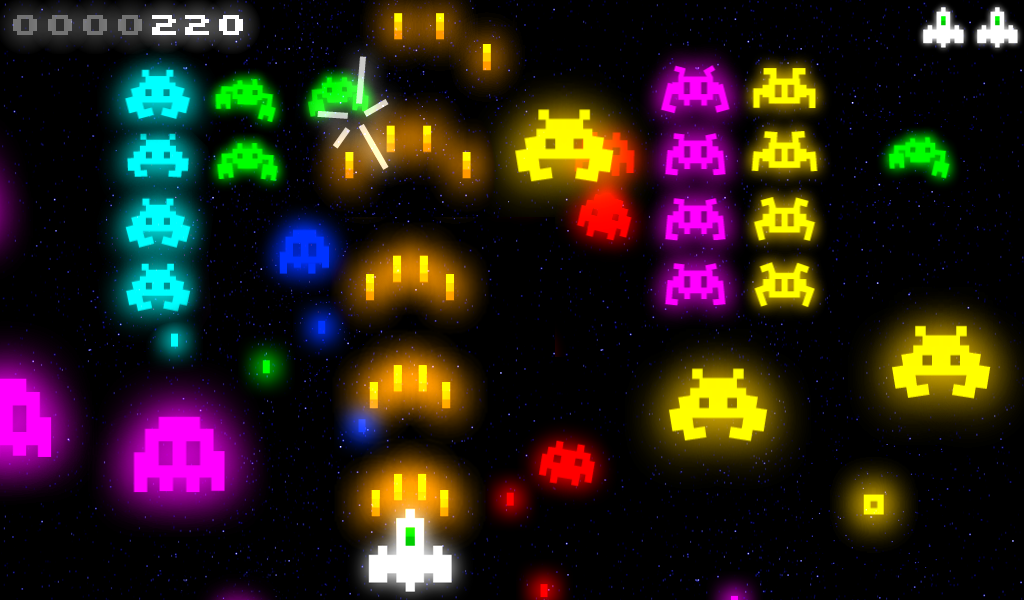
\includegraphics[width=1.0\linewidth]{gameplay.png}
    	\end{figure}
	\section{Overall Design}
		The game which we will build is space invaders. It involves the player controlling a space ship and shooting down aliens. The aliens will fight back with bullets and missiles. The player has a limited number of lives and has to score the maximum in them.
		\begin{enumerate}
			\item The application would be programmed in C++.
			\item The GUI part would involve OpenGL.
			\item UDP sockets will be used for network data transfer.
			\item POSIX threads will be used to run the network and back-end in parallel.
			\item Inter thread synchronization would be done using mutex lock.
		\end{enumerate}

	\section{Sub Components}
		% \begin{enumerate}

			\subsection{Back End}
				TODO: FARAN
				\subsubsection{Alien}
					\begin{lstlisting}[language=C++, caption={Class Parameters for Alien}]
class Alien
{
private:
	float XPos;				// X coordinate
	float YPos;				// Y coordinate
	float Angle;			// Orientation angle
	Color ColorOfAlien;		// Color
	int Level;				// AI difficulty level
	int PresentLives;		// Lives left
	int NumberBullets;		// Bullets fired per shot
	int NumberMissiles;		// Number of missiles left
	int AlienType;			// Type
};
					\end{lstlisting}
				\subsubsection{Ship}
					\begin{lstlisting}[language=C++, caption={Class Parameters for Ship}]
class Ship
{
private:
	float XPos;				// X coordinate
	float YPos;				// Y coordinate
	float Angle;			// Angle
	std::string Name;		// Name of player
	Color ColorOfShip;		// Color of ship
	int Lives;				// Lives left
	int Score;				// Score of player
	int Multiplier;			// Multiplying factor
	int Kills;				// No. of kills
	int Id;					// Player id
	int NumberBullets;		// Bullets fired per shot
	int NumberMissiles;		// Number of missiles left
	int AILevel;			// Level of AI
};
					\end{lstlisting}
				\subsubsection{Color}
					\begin{lstlisting}[language=C++, caption={Class Parameters for Color}]
class Color
{
private:
	float R;				// Value of R component
	float G;				// Value of G component
	float B;				// Value of B component
};
					\end{lstlisting}
				\subsubsection{Bullet}
					\begin{lstlisting}[language=C++, caption={Class Parameters for Bullet}]
class Bullet
{
private:
	float XPos;				// X Coordinate
	float YPos;				// Y Coordinate
	float VelX;				// Velocity X
	float VelY;				// Velocity Y
	Color ColorOfBullet;	// Color
	int ShipId;				// Id of ship fired from
	bool TypeAI;			// If AI bullet
	bool TypePlayer;		// Player type
};
					\end{lstlisting}
				\subsubsection{Board}
					\begin{lstlisting}[language=C++, caption={Class Parameters for Board}]
class Board
{
private:
	std::vector<Ship> VectorShips;		// All ships
	std::vector<Bullet> VectorBullets;	// All bullets
	std::vector<Alien> VectorAliens;	// All aliens
	double DimensionPosX;				// Dimensions + x	
	double DimensionPosY;				// Dimensions + y	
	double DimensionNegX;				// Dimensions - x	
	double DimensionNegY;				// Dimensions - y		
};
					\end{lstlisting}
			\subsection{Artificial Intelligence}
				TODO: KABIR
			\subsection{Graphics}
			% \newline
				TODO: KG
			\subsection{Network Part}
				TODO: SOCCER
	% \newline
	\section{Interaction amongst Sub Components}
		% \subsection{enumerate}
			\subsection{Back-end and UI}
				The GUI will use the data structures directly. The ``Board'' class will be available to generate the display on the screen. The user inputs from keyboard and mouse will be used to generate changes in the class object. 
			\subsection{Back-end and Network}
				TODO KG
	\section{Testing Of Components}
		% \begin{enumerate}
			\subsection{General Unit Tests}
				% \newline
				\begin{lstlisting}[language=C++, caption={Class Parameters for Test}]
class Test
{
private:
	bool verbose;               //If test is to be conducted
	std::string description;    //String description of the test
	bool isPass;                //Boolean if the test has passed 
	void PrintPassFail(bool);   //Prints the status of the test
};
				\end{lstlisting}

				We will use the aforementioned class ``Test'' to perform unit tests on the different files created. This will ensure that all the functions work correctly against some test cases.

			\subsection{Graphics}
				To test the graphics component, we will create aliens and ships at chosen positions. The positions should change appropriately based on user inputs. Bullets should also be fired from the correct positions. When a bullet hits an alien or a ship, proper GUI effects will be added.
			\subsection{Artificial Intelligence}
				TODO KABIR
			\subsection{Network Component}
				TODO SOCCER
			\subsection{Overall Testing}
				For overall testing of the game, we will play the game with as many players as possible and verify the smooth functioning of AI and network component. The network for some clients will be shut down suddenly to check if the transitions for the AI and others are smooth.
	\section{Extra Features}
		\subsection{Competitive Multi-player Mode}
			In this multiplayer mode, the players will be fighting each other. They will try to shoot each other down. Aliens will not be present in this mode. AI players will be present in this.
		\subsection{3D Game-play}
			The game will be taken to 3D in which the aliens and ships can be viewed in a 3D perspective. The camera position will be adjusted by the user based on input from mouse.
		\subsection{Sound Effects}
			Sound effects will be added for the entire game-play. When bullets are fired or some shoot down takes place, appropriate sounds will be played.
		\subsection{Replacement of Player by AI}
			In case of network failures, the player whose network has gone down will get replaced by an AI player of the same level as the player was. This will ensure completely seamless transition in case of network outages. Once the network comes back on, the player will replace the AI control. 
\end{document}
